
		\chapter{Die Magnetische Flussdichte}

Die Magnetische Flussdichte\index{Magnetische Flussdichte} \(B\) ist ein Vektor, mit dessen Hilfe sich berechnen lässt, wie sich ein Magnetisches Feld auf seine Umwelt auswirkt.

		\section{Draht im Magnetfeld} \label{sec1}

Die Magnetische Flussdichte \(B\) gibt an, welche Kraft \(F\) ein Leiter mit der wirksamen Länge\footnote{es ist nur die Länge entscheident, die senkrecht zu den magnetischen Feldlinien steht. Schließt der Draht also den Winkel \(\alpha\) mit den Feldlinien ein, so muss seine wirksame Länge \(s\) berechnet werden mit \(s = s_r \cdot sin(\alpha)\), wobei \(s_r\) die reale Länge des Drahtes ist}~\(s\), der von einem Strom der Stärke \(I\) durchflossen wird, in einem Magnetfeld erfährt.

\begin{equation}
B = \frac{F}{I \cdot s}
\label{Def_B}
\end{equation}
Einheit von \(B\) ist T (Tesla): \(1 T = 1 \frac{N}{A \cdot m}\). Dir Richtung der Kraft \(F\) wird durch die \textit{Linke-Hand-Regel}\index{Linke-Hand-Regel}\footnote{Daumen: physikalischer Stromfluss der Elektronen, Zeigefinger: Richtung der Feldlinien, Mittelfinger: Richtung der Kraft \(F\)} bestimmt.	Diese Kraft wird auch als \textit{Lorentzkraft} bezeichnet (Siehe Kapitel \ref{Lor}).

		\section{langgestreckte Spule}

\index{Näherung für eine langgestreckte Spule}In einer langgestreckten luft- oder materiegefüllten Spule der Länge \(l\) und der Windungszahl \(n\), die von dem Strom \(I_{err}\) durchflossen wird, entsteht ein Magnetfeld mit der Flussdichte

\begin{equation}
B = \mu_0 \cdot \mu_r \cdot I_{err} \cdot \frac{n}{l}
\label{eq_langspule}
\end{equation}
\(\mu_0\) bezeichnet dabei die \textit{Magnetische Feldkonstante}. \(\mu_0 \approx 1,257 \cdot 10^{-6} \frac{V \cdot s}{A \cdot m}\)

\(\mu_r\) bezeichnet dabei die \textit{Permeabilitätszahl}\index{Permeabilitätszahl}. Sie ist der Quotient \(\mu_r = \frac{B_{Materie}}{B_{Vakuum}}\)  Sie hängt zwar von dem Stoff des Spulenkerns ab, ist jedoch keine Stoffkonstante, weil sie auch von der Größe der Magnetischen Flussdichte abhängt.\footnote{\textit{Ferrromagnetische} Stoffe haben \(\mu_r >> 1\), \textit{diamagnetische} Stoffe haben \(\mu_r \approx 1\) und \textit{permamagnetische} Stoffe haben \(\mu_r < 1\). \\ Bsp.: \(\mu_r(Weicheisen) \approx 800, \: \mu_r(Stahl) \approx 4000, \: \mu_r(Permalog) \approx 300000, \: \mu_r(Luft) \approx 1\)}

		\section{Messung der Magnetischen Flussdichte mittels der Hall-Sonde}

In einer Hallsonde\index{Hall-Sonde}, die von einem Strom der Stärke \(I\) durchflossen wird und die die Breite \(d\) in Richtung der Magnetischen Feldlinien des zu messenden Feldes der Flussdichte \(B\) hat, und in der sich \(n\) Elektronen mit der Ladung \(e\) befinden, entsteht die Spannung \(U_H\) senkrecht zu den Magnetischen Feldlinien und senkrecht zur Richtung des Stromdurchflusses.

\begin{equation}
U_H = \frac{1}{n \cdot e} \cdot \frac{B \cdot I}{d}
\end{equation}
Hat die Hallsonde senkrecht zum B-Feld der Stärke \(B\) und zur Bewegungsrichtung mit der Geschwindigkeit \(v\) die Höhe \(h\), so ergibt sich für die Hallspannung \(U_H\):

\begin{equation}
U_H = B \cdot v \cdot h
\end{equation}
Der Hall-Effekt\index{Hall-Effekt} resultiert aus einer Ablenkung der Elektronen aufgrund ihrer Bewegung im zu messenden B-Feld. Dadurch wird Ladung getrennt und es entsteht ein E-Feld. Die Hall-Spannung \(U_H\) stellt sich dann ein, wenn die Ablenkung durch E-Feld (\(F_{el}\)) die Ablenkung durch das B-Feld (\(F_L\)) völlig kompensiert hat.

		\chapter{Lorentzkraft}
		\label{Lor}

Die \textit{Lorentzkraft}\index{Lorentzkraft!Definition} ist eine Kraft, die bewegte Ladungen erfahren, wenn sie sich senkrecht zu den Magnetischen Feldlinien durch ein Magnetisches Feld bewegen. Sie diente uns zur Definition der \textit{Magnetischen Flussdichte} ( \(\rightarrow\) Gleichung \ref{Def_B}).

		\section{Kraft auf einzelne Ladungsträger}

Ein Ladungsträger\index{Lorentzkraft!Auf Ladungsträger} mit der Ladung \(q\), der sich mit der Geschwindigkeit \(\vec{v}\) in einem Magnetfeld der Magnetischen Flussdichte \(B\) senkrecht zu den Feldlinien bewegt, erfährt die Kraft \(F_L\):
	
\begin{equation}
F_L = B \cdot q \cdot v
\end{equation}

		\subsection{Kreisbewegung im Magnetfeld}

Wenn geladene Teilchen in ein Magnetfeld gelangen, bewegen sie sich auf einer Kreisbahn senkrecht zu den Feldlinien des Magnetfeldes. Die Lorentzkraft entspricht dann nämlich der \textit{Zentripetalkraft} \(F_z\) \footnote{\(F_z = \frac{m \cdot v^2}{r}\)}, weil sie immer senkrecht zur Bewegungsrichtung steht und somit ständig zum Kreismittelpunkt zeigt. Der Radius des entstehenden Kreises errechnet sich nach:

\begin{equation}
r = \frac{m \cdot v}{B \cdot q}
\label{eq_kreisbahnrad}
\end{equation}
Das Teilchen hat nach der Zeit \(T\) eine komplette Kreisbahn durchflogen.

\begin{equation}
T = \frac{2 \cdot \pi \cdot m}{B \cdot q}
\label{eq_T}
\end{equation}
Interessanterweise hängt die Umlaufzeit (\ref{eq_T}) nicht von der Geschwindigkeit \(v\) der Teilchen ab. Man macht sich die Erkenntnisse aus (\ref{eq_kreisbahnrad}) zunutze, um die Masse \(m\) der Teilchen\footnote{wenn die Ladung \(q\) Bekannt ist} oder die \textit{speziefische Ladung} \(\frac{q}{m}\)\index{spezifische Ladung} der Teilchen zu messen, da Radius \(r\) und Magnetische Flussdichte \(B\) leicht messbar sind. Damit die Geschwindigkeit der Teilchen zu bestimmen ist, werden sie alle durch einen \textit{Geschwindigkeitsfilter} (\(\rightarrow\) \ref{geschf}) geschickt, wodurch man errechnen kann, wie schnell sie sind.

		\subsection{Schraubenbewegung im Magnetfeld}

Wird das Teilchen so eingebracht, dass seine Geschwindigkeit eine Komponente in Richtung der Feldlinien hat, so bewegt es sich auf einer Schraubenbahn. Schließt die Bewegungsrichtung des Teilchens mit den Feldlinien den Winkel \(\alpha\) ein, so ist die Geschwindigkeit, aus der man den Kreisradius berechnet berechenbar mit \(v_s = v \cdot sin(\alpha)\). Aus der anderen Geschwindigkeit ergibt sich die Längsbewegung der Schraube \(v_l = v \cdot cos(\alpha)\). In der Zeit \(T\) (Siehe \ref{eq_T}) legt das Teilchen dabei längs der Feldlinien die \textit{Ganghöhe} \(h\) zurück. Sie ist der Abstand in Richtung der Feldlinien zwischen zwei Kreisbahnen:

\begin{equation}
h =  \frac{2 \cdot \pi \cdot m}{q \cdot B} \cdot v \cdot cos(\alpha)
\end{equation}

		\section{Geschwindigkeitsfilter}
		\label{geschf}

\begin{figure}[htbp]
	\centering
		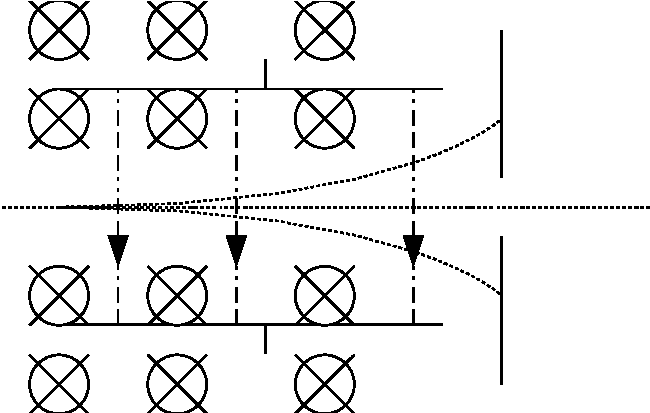
\includegraphics[width=0.42\textwidth]{mat/geschwindigkeitsfilter}
	\caption{Skizze eines Geschwindigkeitsfilters}
	\label{fig:f}
\end{figure}
		
Ein Geschwindigkeitsfilter\index{Geschwindigkeitsfilter} besteht aus einem gekreuzten B-Feld und einem E-Feld. Haben die Teilchen die richtige Geschwindigkeit \(v\), so können sie den Geschwindigkeitsfilter passieren. Der Effekt rührt daher, dass das B-Feld die Teilchen in die andere Richtung ablenkt als das E-Feld. Sind die Teilchen zu schnell, so werden sie vom B-Feld zu stark abgelenkt, sind sie zu langsam, werden sie vom E-Feld zu stark abgelenkt. In Abbildung \ref{fig:f} wirkt die Elektrische Kraft \(F_el\) auf negativ geladene Teilchen nach oben, während die Lorentzkraft \(F_L\) nach unten wirkt. Es gilt dabei:

\begin{equation}
v = \frac{E}{B}
\end{equation}


		\chapter{Elektromagnetische Induktion}

Bei der \textit{Elektromagnetischen Induktion}\index{Elektromagnetischen Induktion} entsteht eine Spannung in einem Leiter, hervorgerufen durch ein Magnetisches Feld. Dies kann auf verschiedene Arten geschehen.

		\section{Relativbewegung}

Bewegt man einen Leiter der Länge \(l\) mit der Geschwindigkeit \(v\) durch ein Magnetfeld der Flussdichte \(B\) (oder das Magnetfeld um den Leiter), so wird in dem Leiter eine Spannung \(U_{ind}\) induziert. Dabei spielt nur die Geschwindigkeitskomponente \(v_s\) senkrecht zu den Feldlinien (und dem Draht) eine Rolle. Für die Richtung des Stromflusses gilt die Linke-Hand-Regel\index{Linke-Hand-Regel}\footnote{Daumen: Bewegungsrichtung des Drahtes, Zeigefinger: Feldlinien, Mittelfinger: Physikalische Stromrichtung}. Es gilt:

\begin{equation}
U_{ind} = v_s \cdot B \cdot l
\end{equation}

		\section{Induktion durch Flächenänderung}
		\label{fland}

Wird eine Leiterschlaufe mit \(n\) Windungen so durch ein homogenes Magnetfeld der Flussdichte \(B\) geführt, dass in der Zeit \(\Delta t\) die vom Feld durchsetzte Schlaufenfläche sich von \(A_1\) auf \(A_2\) ändert\footnote{sich also eine Änderung von \(\Delta A = A_2 - A_1\) ergibt}, so gilt:

\begin{equation}
U_{ind} = n \cdot B \cdot \frac{\Delta A}{\Delta t} = n \cdot B \cdot \dot{A}
\label{eq_fland}
\end{equation}
Durch die Bewegung der Leiterschlaufe am Rande des Magnetfeldes taucht sie also mal mehr und mal weniger ein. Die Flächenänderung kann aber auch als Verformung passieren, oder dass die Leiterschlaufe im Magnetfeld gekippt wird; damit ändert sich nämlich die effektive Fläche, also die Fläche, die zu den Magnetischen Feldlinien senkrecht steht



		\subsection{Sinusspannung}

Somit lässt sich einfach Strom erzeugen, dessen Spannungsverlauf sinusförmig ist. Indem man nämlich eine Spule der Querschnittsfläche \(A_0\) in einem B-Feld rotieren lässt, dass die Rotationsachse senkrecht zu den Feldlinien steht, erhält man eine Fläche \(A_{eff}\) die senkrecht zu den Feldlinien des Magnetfeldes steht, durch die also Induktion stattfinden kann. Es git dabei
\begin{eqnarray}
A_{eff}(t) &=& A_0 \cdot  cos(\varphi) = cos(\omega \cdot t) \\
\dot{A}(t) &=& - A_0 \cdot \omega \cdot sin(\omega \cdot t)
\end{eqnarray}
mit der Kreisfrequenz \(\omega\) und der Zeit der Drehung \(t\), da sich die Spule logischerweise kreisförmig dreht (ihre Seitenkanten beschreiben die Bahn eines Zylinders senkrecht zu den Magentfeldern). Die Flächenänderung \(\dot{A}\) ergibt sich durch die Ableitung nach \(t\). Mittels Formel \ref{eq_fland} kann damit die induzierte Spannung errechnet werden.



		\section{Induktion durch Änderung der Magnetischen Flussdichte}\label{dichland}

In einer Leiterschlaufe mit \(n\) Windungen und der Querschnittsfläche \(A\), die sich senkrecht zu den Feldlinien in einem homogenen Magnetfeld befindet, das in der Zeit \(\Delta t\) von der Flussdichte \(B_1\) auf \(B_2\) geändert wird, ergibt sich:

\begin{equation}
U_{ind} = n \cdot A \cdot \frac{\Delta B}{\Delta t} = n \cdot A \cdot \dot{B}
\label{eq_dichland}
\end{equation}

		\section{Induktionsgesetz}

Kapitel \ref{fland} und \ref{dichland} kann man zu einem einzelnen Gesetz zusammenfassen: Dem \textit{Induktionsgesetz}\index{Induktionsgesetz}. Dafür wird der \textit{Magnetische Fluss} \(\Phi\)\index{Magnetischer Fluss} definiert: Für eine Leiterschlaufe / Spule der Querschnittsfläche \(A\) die sich in einem homogenen Magnetfeld der Flussdichte \(B\) befindet, gilt:

\begin{equation}
\Phi = B \cdot A
\end{equation}
Die Einheit von \(\Phi\) ist \(1 Tm^2 = 1 \frac{N}{A \cdot m} \cdot m^2 = 1 \frac{J}{A} = 1\frac{V \cdot A \cdot s}{A} = 1 V s\)

Möchte man sich \(\Phi\) vernanschaulichen, so kann man sich vorstellen, dass \(\Phi\) die Anzahl der Feldlinien ist, die senkrecht durch die Querschnittsfläche laufen. Die Änderung von einem der beiden Faktoren \(B\) oder \(A\) ruft jeweils eine Induktionsspannung hervor. Kommt in einem Versuch sowohl eine Veränderung von \(A\) als auch von \(B\) vor, so kann man getrennt berechnen, welche Induktionsspannung sich für eine Änderung der durchflossenen Querschnittsfläche ergibt, welche Induktionsspannung sich für die Änderung des B-Feldes ergibt und diese beiden Spannungen addieren, um dann auf die endgültige Induktionsspannung zu kommen. Es gilt also für die Formeln: (\ref{eq_fland}) + (\ref{eq_dichland}) \(\rightarrow\) (\ref{eq_magfl})\footnote{Das hochgestellte Pünktchen bedeutet, dass es sich um eine Ableitung nach der Zeit handelt.}

\begin{equation}
U_{ind} = n \cdot \dot{A} \cdot B + n \cdot A \cdot \dot{B} = n \cdot \dot{\Phi}
\label{eq_magfl}
\end{equation}
Wichtig ist sowohl hier, als auch bei \ref{eq_fland} und \ref{eq_dichland}, dass \(U_{ind}\) zur \emph{Änderung} des Magnetischen Flusses \(\Phi\)
\footnote{also auch zur \emph{Änderung} der senkrecht felddurchsetzten Fläche bzw. der \emph{Änderung} der Flussdichte}
proportional ist. Liegt eine Leiterschlaufe also in einem Magnetfeld, das konstant schwächer wird, so wird eine konstannte Spannung induziert. gleiches gilt, wenn sich die Fläche konstant ändert -- dann wird eine konstannte Spannung induziert.

Zu beachten ist aber auch die Selbstinduktion einer Spule! \(\rightarrow\) Kapitel \ref{selbstind}~!



		\section{Lenz'sche Regel}
		\label{kap_lenzsche_regel}

Die \textit{Lenz'sche Regel}\index{Lenz'sche Regel} besagt, dass ein Induktionsvorgang so verläuft, dass er der Ursache seiner Entstehung entgegenwirkt. 

Wenn also beispielsweise ein Elektromagnet vor einem Metallring eingeschaltet wird, so wird in dem Ring ein solcher Strom induziert, dass das Magnetfeld, welches aus dem Stromfluss im Ring resultiert, entgegen dem der Spule weist.

Die Lenzsche Regel sorgt dafür, dass wir Formel \ref{eq_magfl} abändern müssen:

\begin{equation}
U_{ind} = - n \cdot \dot{\Phi}
\label{eq_lenz}
\end{equation}
Diese neue Induktionsspannung bezieht sich nun auf eine bereits in der Spule bestehende Spannung. Hat man nämlich beispielsweise eine stromdurchflossene Spule und führt in diese Materie ein mit \(\mu_r >> 1\), so sinkt die Stromstärke \(I\) für die Dauer des Einführvorganges. Aus (\ref{eq_langspule}) ist ersichtlich, dass \(B\) steigt. Nach Lenz verläuft die Induktion nun so, dass sie dem Wachstum von \(B\) entgegenwirkt. Ihre Spannung muss also entgegen der "`Urspannung"' sein.

		\section{Selbstinduktion}
		\label{selbstind}

\index{Selbstinduktion}Sobald sich in einer stromdurchflossenen Spule die Stromstärke \(I\) ändert, induziert diese Spule eine Spannung -- eben auch bei sich selbst. Ändert sich nämlich die Stromstärke \(I\) in einer Spule, so sorgt diese Stromänderung für eine Veränderung des Magnetischen Flusses. Aus Kapitel \ref{dichland} folgern wir, dass Induktion stattfinden kann. Diese Induktion findet in der Spule selbst statt, wo eine Spannung induziert wird, die nach der \textit{Lenz'schen Regel} dem Stromfluss, der für die Induktion sorgt, entgegenwirkt. Dabei gilt: \(U_{ind} \sim \dot{I}\). Dieses Phänomen ist als \textit{Selbstinduktion} bekannt. Liegen in einem Stromkreis Schlingungen des Leiters vor, so reagieren diese wie eine Spule.

Die \textit{Induktivität} \(L\) eines Leiters gibt an, wie groß diese entgegengesetzte induzierte Spannung \(U_{ind}\) ist: 
\begin{equation}
U_{ind} = - L \cdot \dot{I}
\label{ind_spule}
\end{equation}
Die Einheit von \(\dot{I}\) ist \(\dot{I} = \frac{A}{s}\)


Die Induktivität\index{Induktivität!allgemein} ist allgemein definiert mit:

\begin{equation}
L = \frac{U_{ind}}{\dot{I}}
\end{equation}
Für \textit{langgestreckte Spulen}\index{Induktivität!langgestreckte Spulen} mit \(n\) Windungen, der Länge \(l\) und mit der Querschnittsfläche \(A\) gilt dabei:

\begin{equation}
L = \mu_0 \cdot \mu_r \cdot n^2 \cdot \frac{A}{l}
\end{equation}
Die Einheit von \(L\) ist : \([L] = \frac{V \cdot s}{A} = \frac{kg \cdot m^2}{C^2} = \frac{kg \cdot m^2}{s^2 \cdot A^2}\)



		\section{Einschaltvorgang eines Spulenstromkreises}
		\label{einschalt}

\index{Einschaltvorgang}Schaltet man einen Stromkreis, in dem eine Spule sitzt, ein, so baut sich die Stromstärke erst mit der Zeit auf. Dies ist ein direktes Resultat der Selbstinduktion. Wenn nämlich der Strom eingeschaltet wird, also in Schaubild \ref{oszi_I} die Funktion sich gerade von der Zeitachse entfernt, ist die Änderung des Stromes \(\dot{I}(t)\) äußerst groß, da sich die Spannung ja von "`überhaupt kein Wert"' auf "`einen positiven Wert"' ändert. Nach Formel \ref{ind_spule} ist die Induktionsspannung hier also stark negativ. Mit dem \textsc{Lenz}'schen Gesetz in Einklang ist diese Induktionsspannung also ihrer Ursache entgegengesetzt und "`\textit{fängt}"' die Veränderung der Stromstärke ab. Der Stromverlauf ist deshalb an dieser Stelle auch kurvenförmig. Ohne die entgegengerichtete Induktionsspannung hätte der Strom sein Maximum praktisch sofort erreicht. So nährt er sich seinem Maximum nur \textit{asymptotisch} an.

Je mehr Zeit innerhalb einer halben Periode verstreicht, desto näher kommt der ausgebremste Strom seinem Maximum, aber immernoch ist eine gegenläufige Spannung da, die ihn dezimiert. Da er konsequent dezimiert wird, wird \(\dot{I}(t_n)\) auch kleiner, da ja ständig die wachstumsschwächende Induktionsspannung auf den Strom einwirkt.

Wenn der Strom dann wieder abgeschaltet wird, also von seinem Maximum abfällt, ist in Schaubild \ref{oszi_U} ein noch größerer Peak\index{Peak} entstanden, der diesmal nach oben zeigt, also auch eine große positive Spannung hinweist. \(\dot{I}(t_n)\) ist an dieser Stelle stark negativ, weil der Strom sich von einem nahezu konstannten Wert "`\textit{erstmalig}"' abbewegt. Nach Gleichung \ref{ind_spule} sorgt diese Spannung nun dafür, dass der Stromstärkenabfall abgefangen wird, also nicht so drastisch aussieht, weshalb sich auch hier wieder ein kurvenförmiger Lauf ergibt.


\begin{figure}[h]
\centering
\subfigure[Stromverlauf]{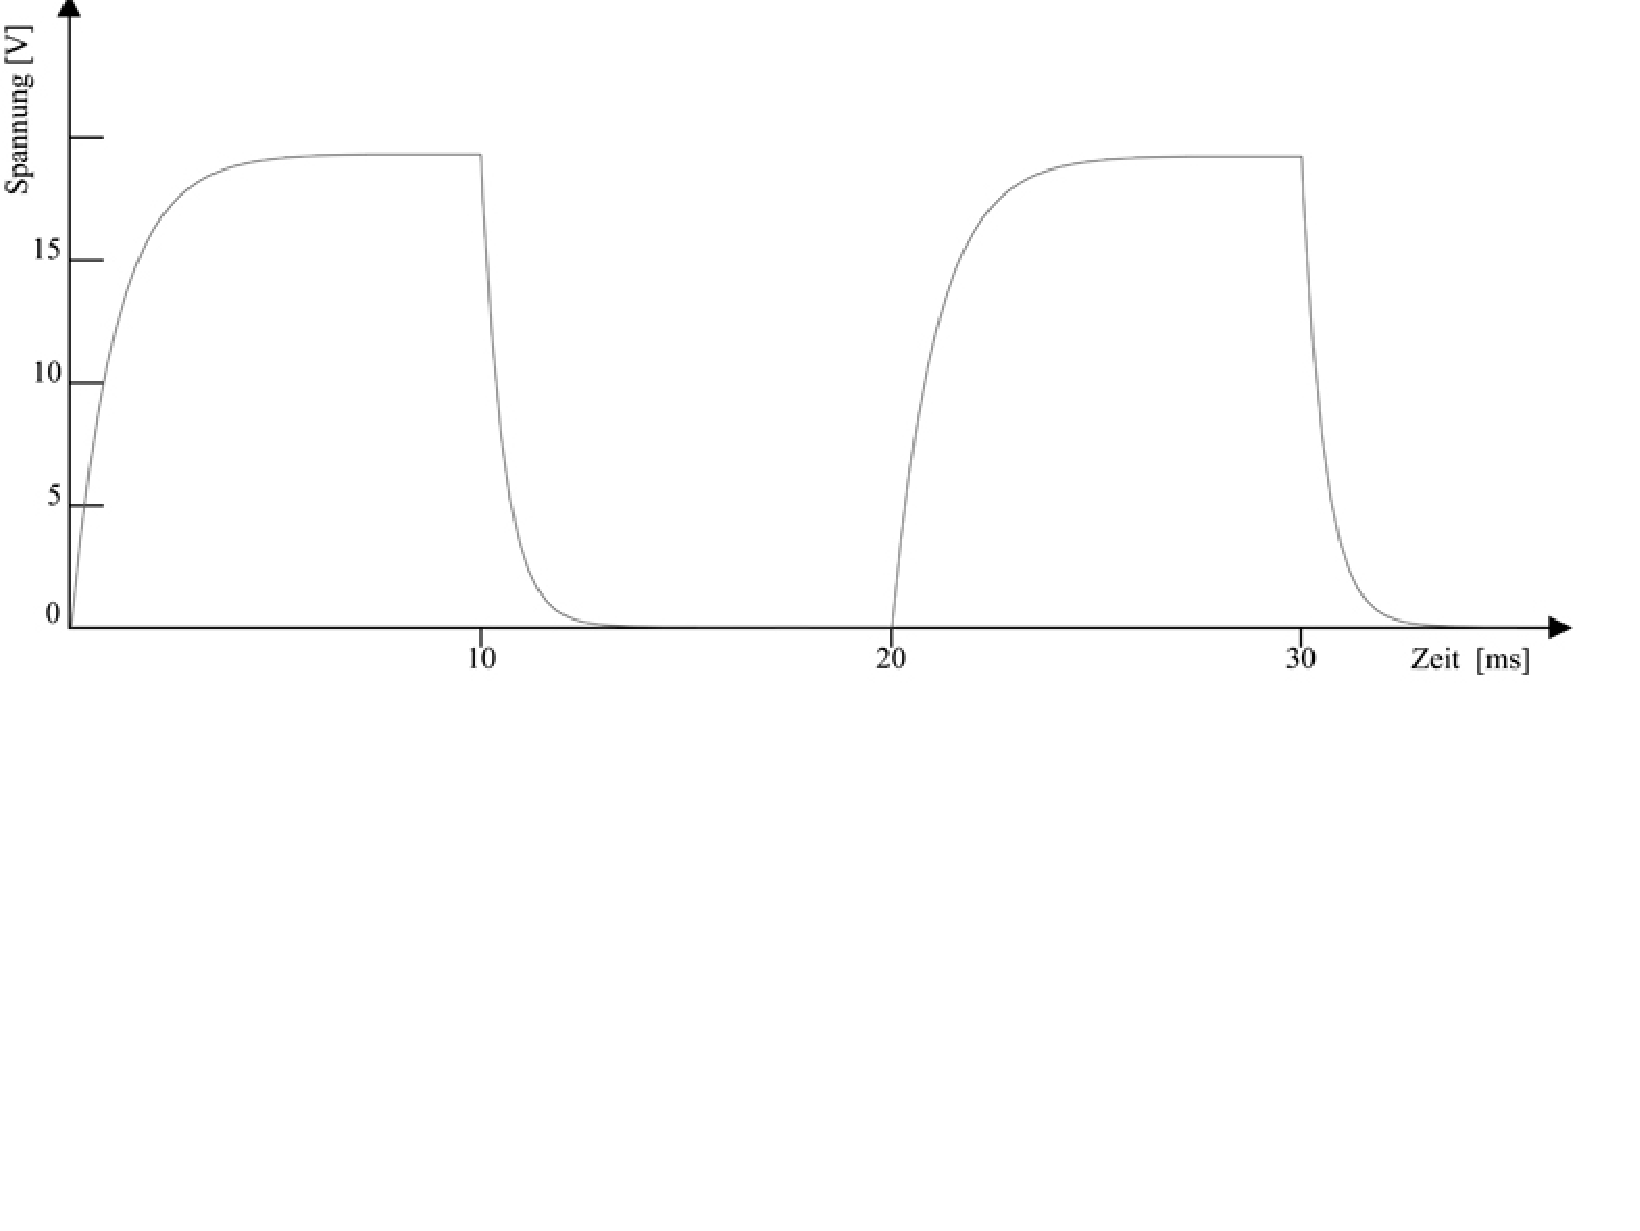
\includegraphics[width=0.45\textwidth]{mat/oszi_I}\label{oszi_I}}
\subfigure[Spannungsverlauf]{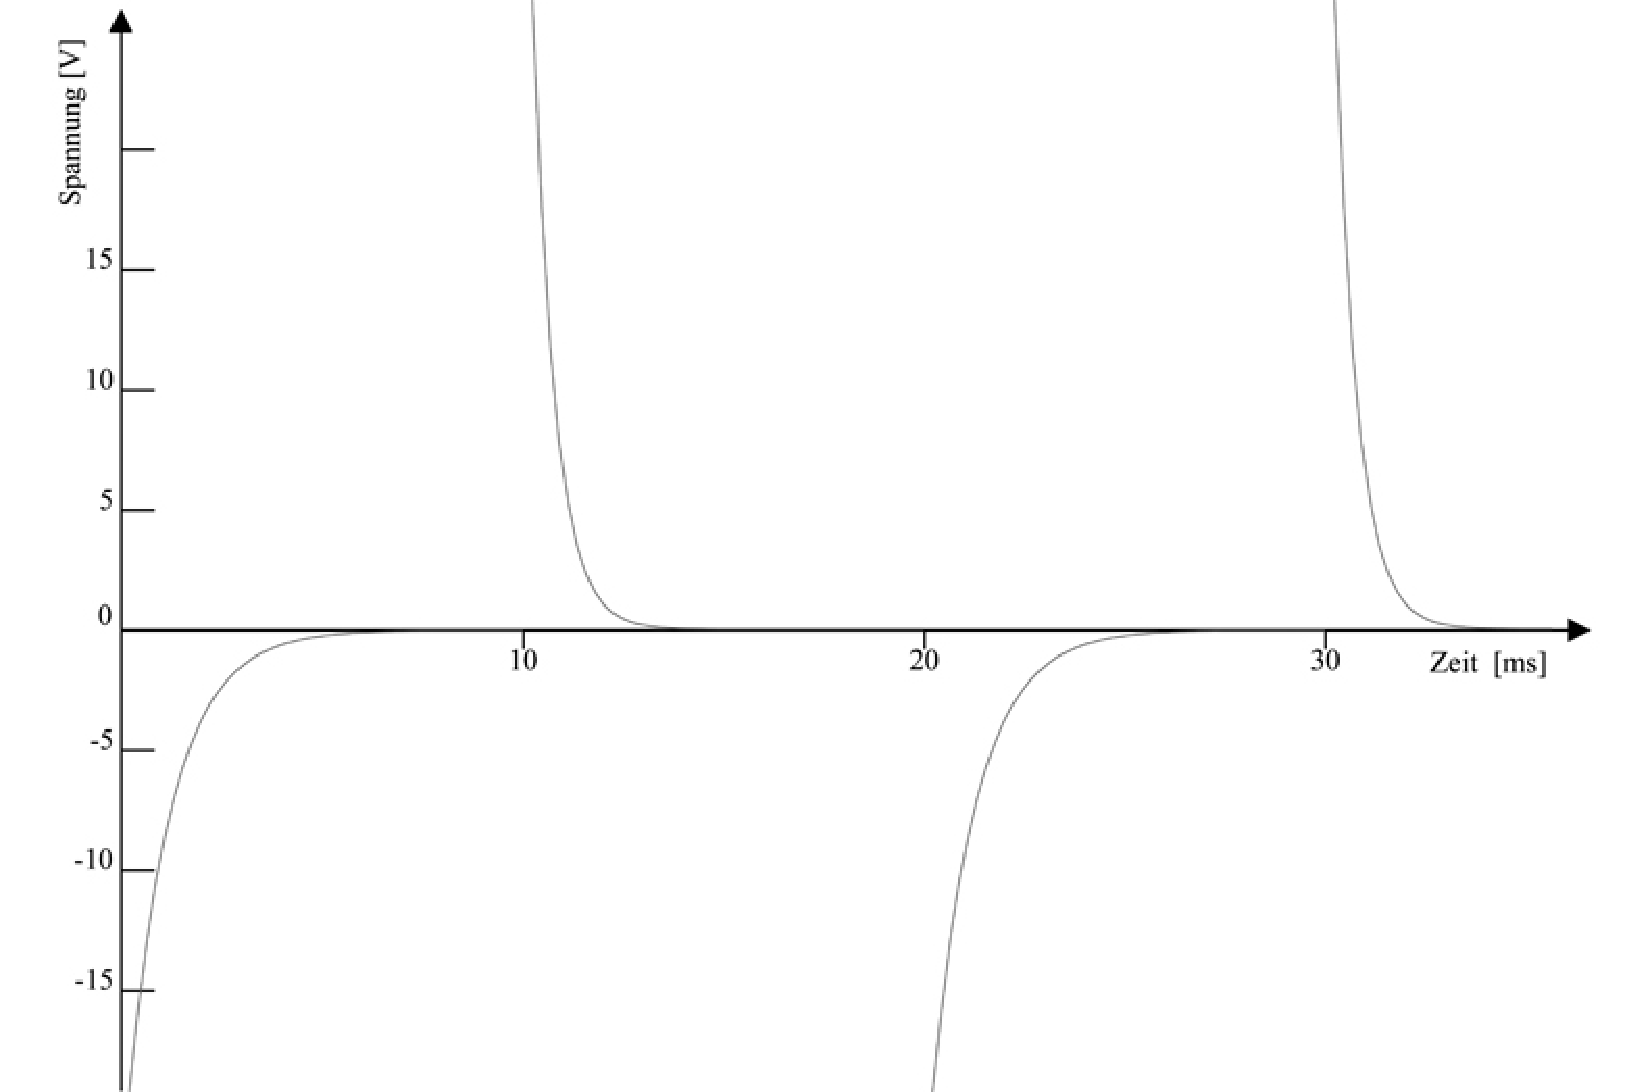
\includegraphics[width=0.45\textwidth]{mat/oszi_U}\label{oszi_U}}
\caption{Vorgänge beim Einschalten eines Stromkreises mit Spule -- siehe Kapitel \ref{einschalt}}
\label{oszi}
\end{figure}



		\section{Energie des Magnetfelds}

Unterbricht man einen Spulenstromkreis, so wird die Spule nach dem \textsc{Lenz}'schen Gesetzt dafür sorgen, dass der Strom noch möglichst aufrecht erhalten wird. Mit diesem Strom kann Arbeit verrichtet werden -- im Magnetfeld muss also Energie gespeichert sein. Die enthaltene Energie des Magnetfeldes zwischen zwei Zeitpunkten \(t_1\) und \(t_2\) berechnet sich mit
\begin{equation}
E_{mag} = \int_{t_1}^{t_2} P(t) dt
\label{int_Emag}
\end{equation}
Mit der Formel für elektrische Leistung \(P_{el} = U \cdot I\) und Formel \ref{ind_spule} ergibt sich so\footnote{Weil \(\dot{I} = \frac{dI}{dt}\) und somit \( \dot{I} \cdot dt = \frac{dI}{dt} \cdot dt = dI\)}
\begin{equation}
E_{mag} = - \int_{t_1}^{t_2} \left ( L \cdot \dot{I}(t) \cdot I(t) \right ) dt = 
- \int_{I(t_1)}^{I(t_2)} \left ( L \cdot I(t) \right ) dI(t) = 
- L \left [ \frac{1}{2} \cdot I^2 \right ]_{I(t_1)}^{I(t_2)}
\label{e_mag}
\end{equation}


% 		\chapter{Definitionen, Größen}
%
% \begin{description}
% 	\item[\(\frac{q}{m}\)] bezeichnet die \textit{Spezifische Ladung} eines Teilchens. Für Elektronen gilt: \( \frac{e}{m}~=~1,7588~\cdot~10^{11}~\frac{C}{kg}\)
% 	\item[\(\mu_r\)] bezeichnet die \textit{Permeabilitätszahl}, die festlegt, um wie viel stärker das Magnetfeld wird, wenn man einen Materiekern einführt.
% \end{description}
